\documentclass[10pt]{article}
%\usepackage[latin1]{inputenc}
%\usepackage[english]{babel}
\usepackage[dvips]{graphicx}

\usepackage{amssymb}
\usepackage{amsfonts}
\usepackage{amsmath}

\newcommand{\lio}{\textsf{lio}}
\newcommand{\ttu}{\textsf{ttu}}
\newcommand{\vlio}{\textsf{vlio}}
\newcommand{\vttu}{\textsf{vttu}}
\newcommand{\alio}{\textsf{alio}}
\newcommand{\attu}{\textsf{attu}}

\newcommand{\overall}{\emph{overall}}
\newcommand{\spka}{\emph{spk5vs1}}
\newcommand{\spkb}{\emph{spk3vs3}}
\newcommand{\spkc}{\emph{spk1vs5}}
\newcommand{\coa}{\emph{coart4vs1}}
\newcommand{\cob}{\emph{coart3vs2}}

\begin{document}

\begin{center}
\section*{Supporting Information Text}
\end{center}

\section{Data Set}

\subsection{Subjects and Set-up}

Six female Italian native speakers were recorded while uttering
Italian words and pseudo-words.
 Words were mainly stress-initial, e.g.,
"matto", "nome", "strada" ("mad","name", "road"), and were chosen in order
to have consonants both at the beginning and in the middle of
words, followed by different vowels and consonants.

The data recording setup included a \emph{Laryngograph Microprocessor}
device (Laryngograph Ltd., London, www.laryngograph.com) which gathers speech audio
signal and the electroglottographic (EGG) signal at $16$KHz sampling
rate; and an AG500 electromagnetic articulograph (Carstens Medizinelektronik
GmbH, Germany, www.articulograph.de) that records the
3D positions of a set of sensors glued on the tongue, lips and front teeth
during speech production at a sampling rate of $200$Hz. 

A full description of the 
acquisition set-up and the obtained database can be found in \cite{tavella}.

\subsection{Phone Segmentation}
In order to carry out a speech segmentation based on the motor invariants of the consonants under
examination we first formally define those invariants:

\begin{itemize}

  \item Let $s_1(t)$ and $s_2(t)$ be the signals associated
    with sensors placed on two phonetic actuators (e.g., the upper and
    lower lips), and $\delta(t) = ||s_1(t)-s_2(t)||$ be their
    Euclidean distance. Then, a plosion is defined as the interval
    between two instants $t_{start}$ and $t_{end}$ such that
    $\dot{\delta}(t_{start}) = 0 $ and $\ddot{\delta}(t_{start}) > 0$,
    and $\dot{\delta}(t_{end}) > 0 $ and $\ddot{\delta}(t_{end}) = 0$.

  \item For the bilabial consonants /b/ and /p/, the sensors on the upper and lower
    lip are considered for $s_1(t)$ and $s_2(t)$, whereas for the labio-dental /d/ and /t/
    those on the tongue tip and upper teeth are. In turn, the associated
    distances will be denoted as \lio\ (lips opening) and \ttu\
    (tongue tip - upper teeth distance). As well, the respective velocities
    and accelerations will be denoted by \vlio, \vttu, \alio, \attu.

\end{itemize}

Then the segmentation is carried out as follows: for each
utterance, all sequences matching the conditions defined above
are displayed and the associated speech is played, so that the experimenter 
can choose whether the
sequence is a correct guess or it is a false positive.

 In this experiment we only
monitor \lio\ and \ttu, so that false positives appear, e.g., when considering
/ts/ and /dz/. This is why, at this stage, a completely automatic segmentation
cannot be enforced. If the sequence is accepted, it is labelled
with the associated consonant, the speaker, and the
coarticulating phoneme. For example, from the word /bronzo/ (bronze) a /b/
sequence is extracted, and the letter "r" is stored as the coarticulating phoneme.
This way, from the original $77$ words and pseudowords, a total
of $1157$ audio/motor sequences are extracted, with a length of $122 \pm 41.2$
milliseconds (mean $\pm$ one standard deviation), minimum length $50$ milliseconds,
maximum length $335$ milliseconds.

\section{The Audio-Motor-Map}
\subsection{Neural Network Training}

A feed-forward neural network is set up in order to
build the AMM, with $380$ input units, one hidden layer with $15$ units and
$4$ output units; the net is trained via the Scaled Conjugate Gradient
Descent method \cite{MOLLER93} and the activation is a logistic sigmoidal function.

Training is done via early stopping on the appropriate validation set.
This procedure is repeated over $10$ random restarts, and then
the network with best average performance over the $4$ output dimensions is stored.
The performance measure is Matlab's embedded mean-square-error with regularisation
function, in which after some initial experiments we set the regularisation
parameter at $0.714$. This value, as well as all other parameters, have been found in
an initial experimentation phase, by slightly altering values suggested in literature
and/or in the Matlab manual.

No sample normalisation is performed, in order to preserve the time structure of the
spectrogram windows. Targets are normalised in order to lie within the range $[0.1,0.9]$,
since the logistic activation function has asymptotic values of $0$ and $1$.

\section{Phoneme Discrimination}
\subsection{Feature Sets - Audio Feature Set}

``Audio'' is a set of $390$ cepstral coefficients extracted from the audio signal
as follows. We consider a set of $25$-milliseconds long ``time slices'' of the signal.
From each slice $13$ cepstral coefficients, plus their first- and second-order derivatives,
are evaluated using a Mel-scale filterbank comprising $29$ filters in the bandwidth from
$20$Hz to $2$KHz; this results in $39$ coefficients for each slice. This is a state-of-the-art
set of features according to recent literature \cite{bourl,pinto:icassp-phnrecog:2008}
in which the single slices are classified as belonging to a phoneme or another with a certain
probability, and then a time-sequence probabilistic method (typically, a Hidden Markov Model)
is used. In our case, a whole variable-length sequence must be classified, so we consider
$10$ slices uniformly distributed across the sequence itself in order to cover it completely.
In case the sequence is shorter than $250$ milliseconds, the slices are allowed to overlap,
whereas in the opposite case there are gaps between them.

\subsection{Feature Sets - Real Motor Feature Set}
``Real motor'' is a set of $16$ coefficients evaluated as follows: for each
signal considered (\vlio, \alio, \vttu\ and \attu), a least-squares piecewise
Hermite cubic interpolation is generated over the sequence. This results in $4$ real
numbers per signal (constant, I-, II- and III-order coefficient of the cubic
interpolant). The choice of interpolating the signal trajectories is motivated by
the need to capture the qualitative (plosive, in this case) behaviour of the sensors
abstracting away from, e.g., the length of the plosion, and to compactly represent it.
Preliminary manual inspection of the trajectories has convinced us that a cubic fit
would adequately capture their shapes.

\subsection{The Support Vector Machine-based classifier}
The classifier is a Support Vector Machine \cite{BGV92} with Gaussian kernel
and hyperparameters $C, \sigma$ found by grid-search. Samples are normalised
by subtracting the mean values and dividing by the standard deviations,
dimension-wise, in the real motor and reconstructed motor cases, while
no normalisation is applied to the audio features. The off-the-shelf SVM
package \emph{libsvm} \cite{libsvm} has been used.

Support Vector Machines output decisions but not the probabilities of their 
decisions, i.e., the posterior probabilities. Only approximate estimations of 
the posterior probabilities can be computed. The \emph{libsvm} implementation provides these
estimations (see \cite{libsvm}) that are necessary for the "Joint feature set" based classifier.

\begin{thebibliography}{99}

\bibitem{tavella}
M.~Grimaldi, B.~Gili~Fivela, F.~Sigona, M.~Tavella, P.~Fitzpatrick,
  L.~Craighero, L.~Fadiga, G.~Sandini, and G.~Metta.
\newblock New technologies for simultaneous acquisition of speech articulatory
  data: 3{D} articulograph, ultrasound and electroglottograph.
\newblock In {\em Proceedings of LangTech 2008, Rome, Italy}, 2008.

\bibitem{MOLLER93}
Martin~F. Moller.
\newblock A scaled conjugate gradient algorithm for fast supervised learning.
\newblock {\em Neural Networks}, 6:525--533, 1993.

\bibitem{bourl}
P.~Pujol, A.~Hagen, H.~Bourlard, and C.~Nadeu.
\newblock Comparison and combination of features in hybrid {HMM/MLP} and
  {HMM/GMM} speech recognition.
\newblock {\em IEEE Transactions of Speech and Audio Processing},
  13(1):14---22, 2003.

\bibitem{pinto:icassp-phnrecog:2008}
Joel~Praveen Pinto, Hynek Hermansky, B.~Yegnanarayana, and Mathew
  Magimai.-Doss.
\newblock Exploiting contextual information for improved phoneme recognition.
\newblock In {\em "{IEEE} Int. Conf. on Acoustics, Speech, and Signal
  Processing ({ICASSP})"}, 2008.

\bibitem{BGV92}
B.~E. Boser, I.~M. Guyon, and V.~N. Vapnik.
\newblock A training algorithm for optimal margin classifiers.
\newblock In D.~Haussler, editor, {\em Proceedings of the 5th Annual ACM
  Workshop on Computational Learning Theory}, pages 144--152. ACM press, 1992.

\bibitem{libsvm}
Chih-Chung Chang and Chih-Jen Lin.
\newblock {\em {LIBSVM}: a library for support vector machines}, 2001.
\newblock Available at http://www.csie.ntu.edu.tw/\~{}cjlin/libsvm.

\end{thebibliography}

\end{document}

\begin{center}
\section*{Supporting Figures}
\end{center}

%figure S1
\begin{figure*}[hb]
  \centerline{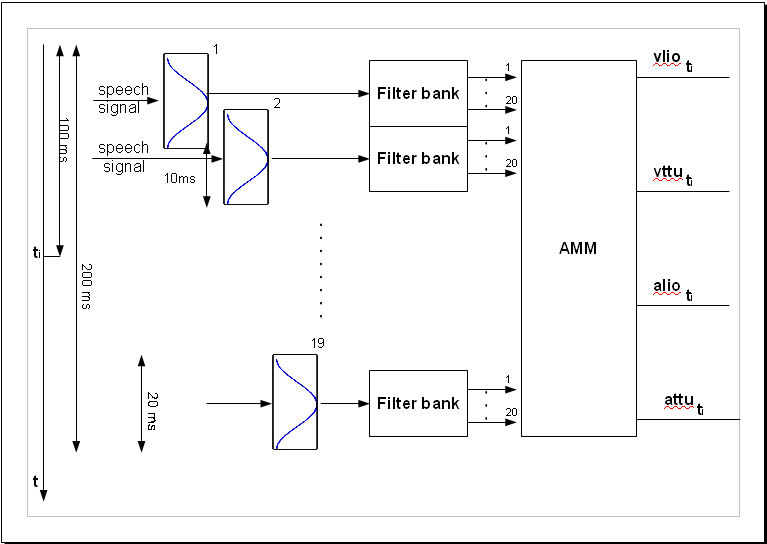
\includegraphics[width=\textwidth]{figs/audio2motor}}
\renewcommand{\figurename}{Figure S}
 \caption{From speech signal to reconstructed motor information. To reconstruct
   a single sample of \vlio, \alio, \vttu\ and \attu\ at time $t_i$ the
  spectrogram of nineteen $20$-millisecond long Hamming windows is evaluated.
   One window is centered at time $t_i$, $9$ windows precede it
   and $9$ windows follow it. Each window overlaps by $10$ milliseconds
  with the preceding window. The spectrogram is computed by using a
   $20$-filter Mel-scale filterbank.}
 \label{fig:amm}
\end{figure*}


%figure S2
\begin{figure*}[hb]
\renewcommand{\figurename}{Figure S}
 \centerline{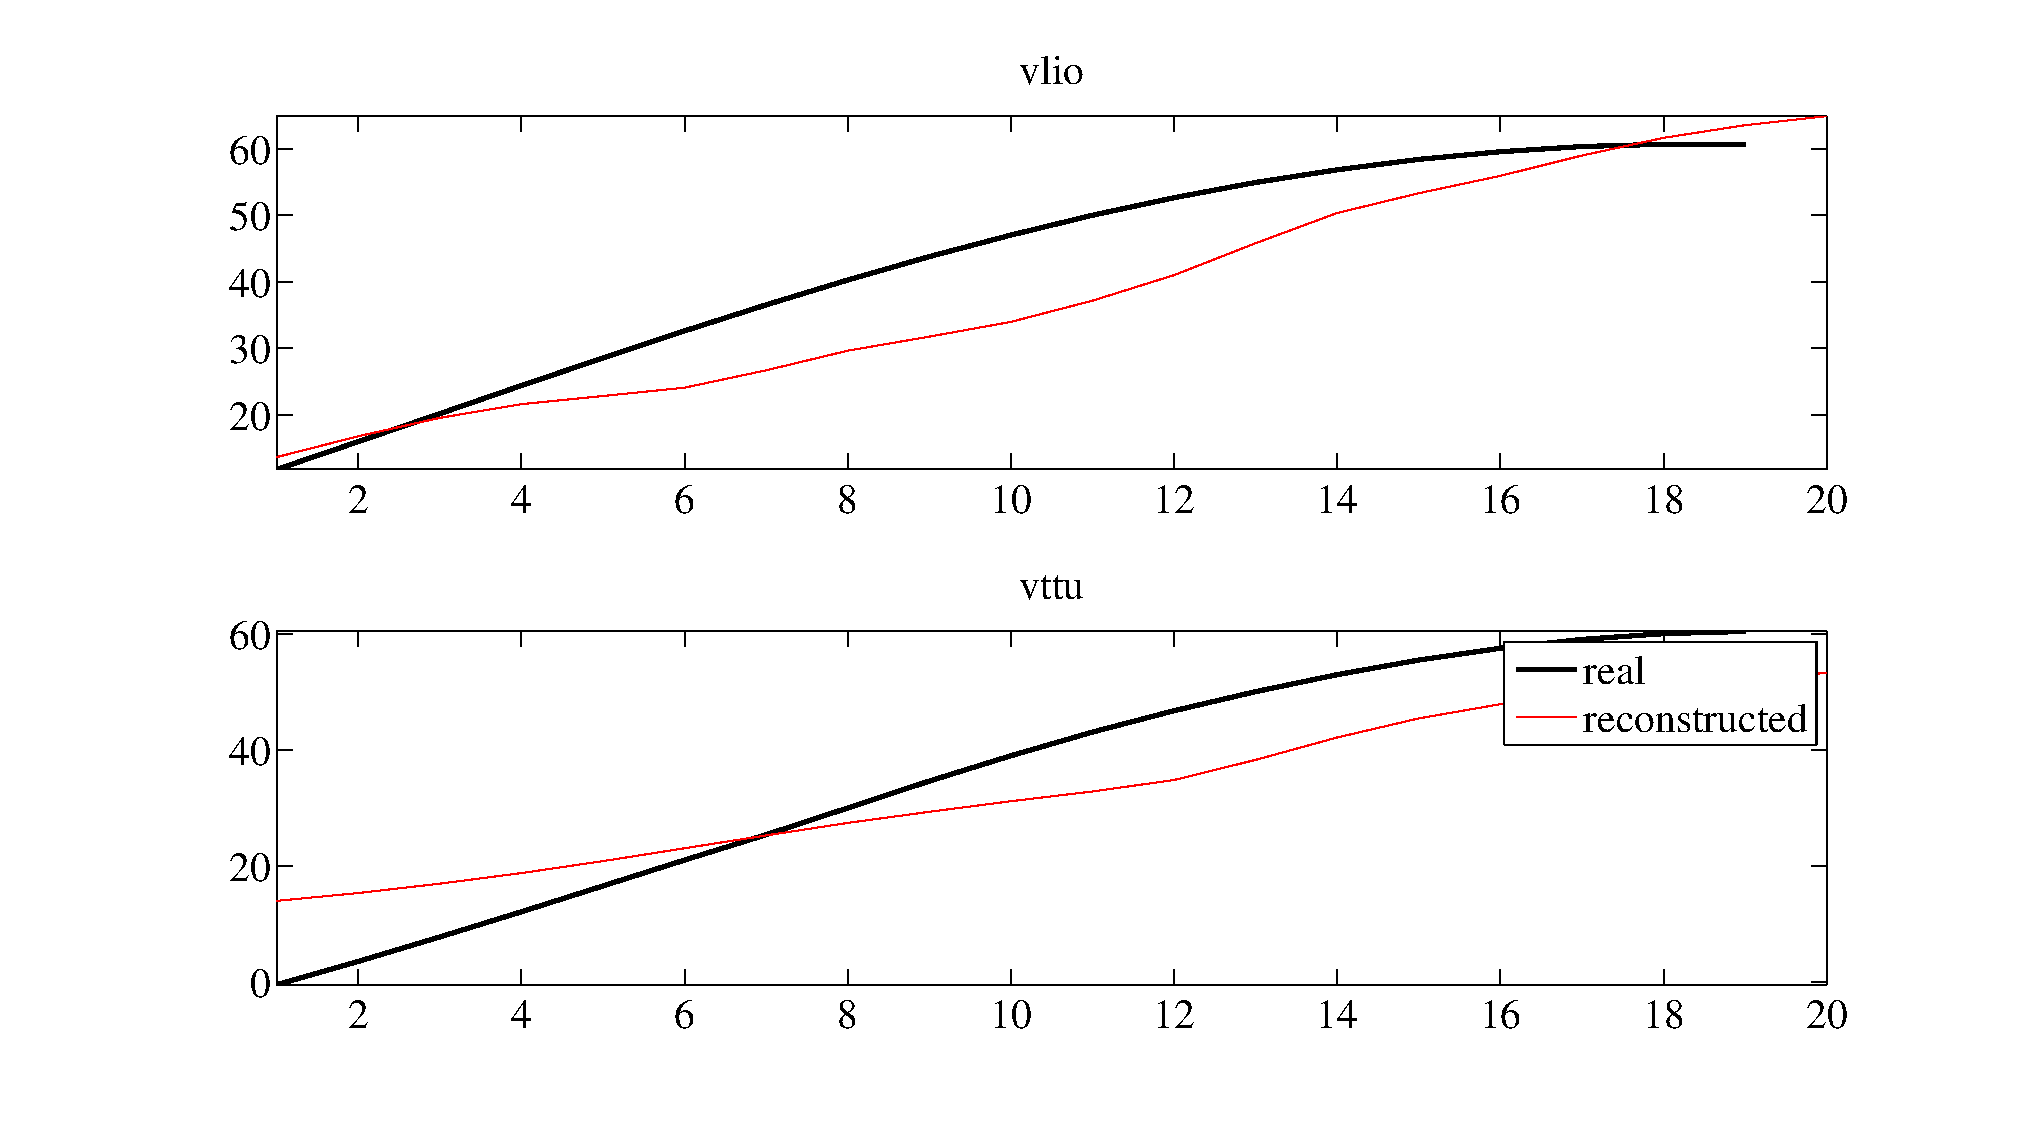
\includegraphics[width=\textwidth]{figs/recMIs}}
 \caption{Real and AMM-reconstructed \vlio\ and \vttu\ for subject $6$ uttering
    the /t/ in \emph{accento?} (accent). Notice the apparent gap in the quality
   of the reconstruction, favouring in this case the labiodental trajectory (\vttu).}
 \label{fig:example}
\end{figure*}

%figure S3
\begin{figure*}[t]
\renewcommand{\figurename}{Figure S}
  \centerline{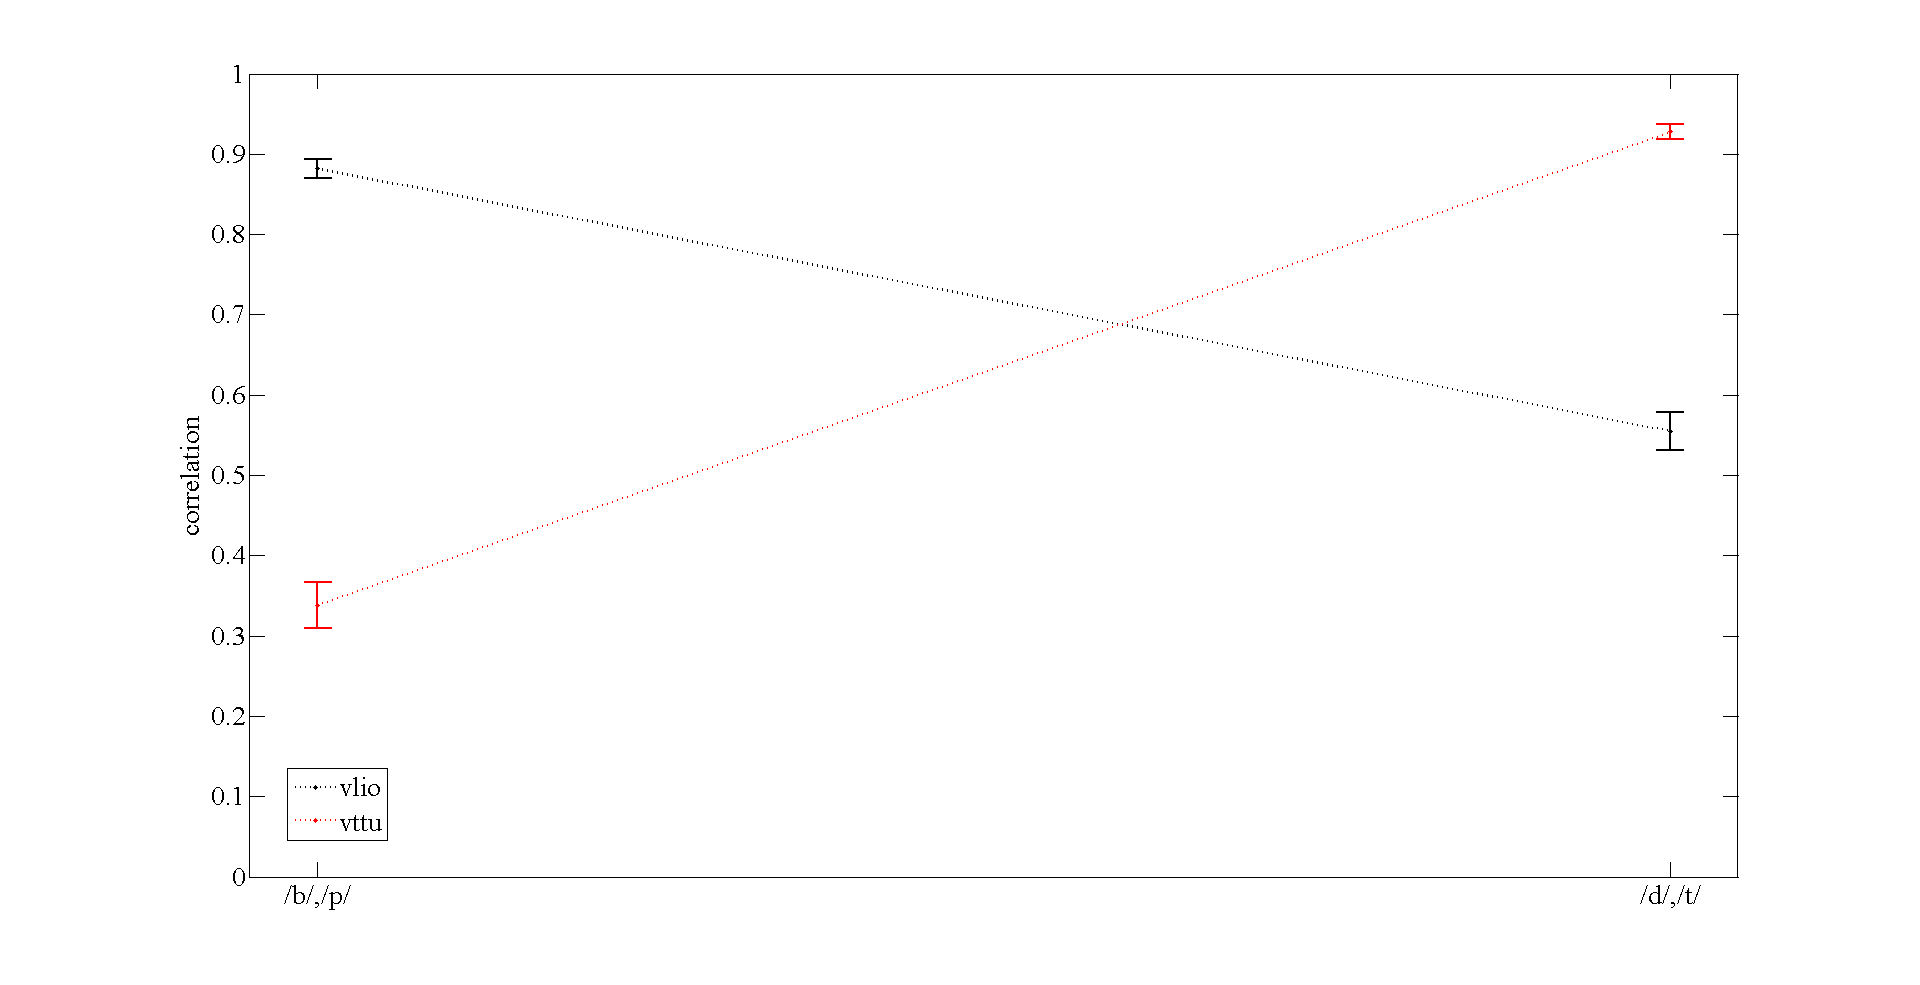
\includegraphics[width=\textwidth]{figs/doubleDiss}}
  \caption{Double dissociation of correlation between real and AMM-reconstructed MI
    (mean and standard error of the mean). Mean coefficients are significantly
    higher for \vlio\ when ``listening'' to labials than dentals and vice-versa.
    The \overall\ CV schema is used.}
  \label{fig:DD}
\end{figure*}